%! Author = jacobcarlson
%! Date = 4/25/23

% Preamble
\documentclass[]{article} %twocolumn
% Packages
\usepackage{amsmath}
\usepackage{algorithm}
\usepackage{algorithmic}
%\usepackage{algorithmicx}
\usepackage{graphicx}
\usepackage[margin=1in]{geometry}
\usepackage{siunitx} % Required for alignment
\usepackage{caption}
\usepackage[style=numeric,natbib=true]{biblatex}
\usepackage{authblk}

\sisetup{
  round-mode          = places, % Rounds numbers
  round-precision     = 2, % to 2 places
}
%\usepackage{biblatex}
%\usepackage{algpseudocode}


\graphicspath{ {./images/} }
\addbibresource{chapters/sources.bib}

\title{
    Experiments on Recognition of Malware based on Static Opcode Occurrence Distribution\\
}
\author[1]{Jacob Carlson}
\author[1]{Anca Ralescu}
\author[2]{David Knapp}
\author[2]{Temesguen Kebede}
\affil[1]{University of Cincinnati}


\affil[2]{AFRL}

% Document
\begin{document}

    \maketitle

%    \tableofcontents
%    \newpage

    %! Author = jacobcarlson
%! Date = 4/27/23

\section*{Abstract}
This paper discusses a static method for recognizing malicious code samples by comparing opcode distributions created
through a novel approach.
Distributions are created by aggregating the number of operations between consecutive calls
of an opcode.
Creating these distributions for each file and comparing them to ground truth distributions representing
benign and malicious code samples creates a set of input values that can lead to an accurate
method of malicious code detection.
This paper also provides a dataset of distributions, as well as describes the methods used to create these distributions.

\section*{Keywords}
Opcode Distributions, Opcode Dataset

\section*{Acknowledgment}
The work of the first author was partially supported by AFRL under contract AFRL-1234-5678.
This was PA cleared PA \#123 (CHANGE PLACEHOLDERS)
    %! Author = jacobcarlson
%! Date = 4/26/23



\section{Proposed Plan}

Static malware analysis is an approach in which an executable is inspected for malware without being executed. The
most common methods include matching common patterns or deriving a series of parameters to learn from each file,
such as the Ember Data set\cite{ember}.
This paper proposes a method of static malware analysis in which an executable will be translated into a set of distributions that will be compared against ground truth distributions from both
benign and malicious code samples.
These comparisons will then be used to determine whether a file is malicious or
benign.

All compiled code exists as a sequence of op codes, instructing the machine on what to do at the most basic level.
While the sequence in which the opcodes are written is not the exact same order in which they will be executed, it
is still a very strong representation of the program at hand.
To create a set of distributions for an executable,
the number of operations between occurrences of the same opcode will be obtained for each common opcode.
This data is then placed into bins and divided by the total number occurrences to create an empirical
probability distribution of the occurrences of each tracked opcode.

This distribution will then be compared to ground truth distributions using the Kullback-Leibler divergence to
assess the difference between distributions.
These KL divergence values will then be used as input data in a machine learning model to detect the
presence of malicious code in an executable.


    %! Author = jacobcarlson
%! Date = 4/25/23

\section{Data Acquisition}

To train a network capable of detecting malicious code, a large dataset was needed. Most online datasets for malware
detection do not provide raw files in their datasets, especially at scale; however, Practical Security Analytics,
an online security blog, has released a dataset of $200,000+$ benign and malicious executables for machine learning
purposes\cite{lester}.

This analysis focuses on the instructions that a machine will execute, so Unix command $objdump\; -d$ was used to
disassemble the executable into a human readable form that lists the instructions as they would be received by the
operating system executing them. This form provides more than the opcode being executed, so extra information such
as the line number and the parameters of the instruction must be removed. Each instruction follows a common form,
so python was used to filter each entry down to its opcode. To remove the risk of the executable being used and
simplify data access, opcode lists will then be stored and used for future operations instead of the executable form.


    \section{Distribution Construction}

\subsection{Single Executable Distribution Construction}

In this method, the final goal is to have a set of distributions that can be compared to ground truth distributions to
determine whether or not the file contains malicious code.
Distributions are created by taking all the jumps between occurrences of a given op code, $op$, and aggregating it in
$b$ bins using the bin assignment function $\phi$ to discretize the data.
A jump is the number of instructions invoked between two opcodes of the same type.
Given the executable file has been converted to an opcode sequence, the indices of each opcode in the list can
be used to determine the jumps between successive op codes.
The construction of a single executable distribution set is shown in Algorithm \ref{alg:algorithm_single}.

\begin{center}
    $bin \; assignment:\; \phi(jump) = \lfloor \frac{jump}{1000} * bin_{size} \rfloor$
\end{center}

Since executables are of variable length, and it is possible for a jump to be close to the length of the entire
executable if occurrences are sparse, jump values are capped at 1000 to reduce extreme outliers.
These large jumps are infrequent, so keeping them would skew the distributions and subsequent comparisons to
such distributions.
Any jump value whose bin assignment falls outside the number of bins is omitted.

%! Author = jacobcarlson
%! Date = 4/26/23

\begin{algorithm}
    \caption{Single Executable Distribution Algorithm}
    \begin{algorithmic}
%        \STATE  $\mathrm{train\_ANN} (f_i,w_i,o_j)$
        \FOR{$op$ in opcode set}
            \STATE $N_{op} \gets $ number of op occurrences
            \STATE $distribution_{op} \gets 0$ vector the size of the number of bins
            \FOR{each occurrence of $op$ in sequence = $1$ to $(N_{op}-1)$}
                \STATE $jump_{op\_k} = op_{k+1} - op_{k}$
                \STATE $distribution_{op}[\;\phi(jump_{op\_k})\;]$ += 1
            \ENDFOR
            \FOR{each bin $b$ in $distribution_{op}$ = $1$ to $B$}
                \STATE $distribution_{op}[b]$ \textbackslash= $(N_{op}-1)$
            \ENDFOR
        \ENDFOR
    \end{algorithmic}\label{alg:algorithm_single}
\end{algorithm}

\subsection{Multiple Executable Distribution Construction}
The process to create aggregated distributions is similar to the algorithm for individual files, with the exception that
the distribution is aggregated over a large number of files of the same class.
By only aggregating files over one class, distribution sets are created that are representative of what a typical
jump distribution from a single executable should look like.
The construction of a multiple executable distribution set is shown in Algorithm \ref{alg:algorithm_multiple}.

The values obtained from comparing a code sample to a ground truth distribution of each class over all opcodes in
an opcode set will generate a vector of values twice the size of the opcode set, each distribution is compared to a
benign and malicious ground truth.
This will be used as the input to machine learning models for each sample.

%! Author = jacobcarlson
%! Date = 4/26/23

\begin{algorithm}
    \caption{Multiple Executable Distribution Algorithm}
    \begin{algorithmic}
        \FOR{$op$ in opcode set}
            \STATE $distribution_{op} \gets 0$ vector the size of the number of bins
        \ENDFOR
        \FOR{executable $l$ = $1$ to $L$}
            \FOR{$op$ in opcode set}
                \STATE $N_{l\_op} \gets $ number of op occurrences in $l$
                \FOR{each occurrence of $op$ in sequence = $1$ to $(N_{l\_op} - 1)$}
                    \STATE $jump_{l\_op\_k} = op_{l\_k+1} - op_{l_k}$
                    \STATE $distribution_{op}[\;\phi(jump_{l\_op\_k})\;]$ += $1$
                \ENDFOR
            \ENDFOR
        \ENDFOR
        \FOR{$op$ in opcode set}
            \STATE $total\_jumps_{op} \gets \sum_{b=1}^B distribution_{op}[b]$
            \FOR{each bin $b$ in $distribution_{op}$ = $1$ to $B$}
                \STATE $distribution_{op}[b]$ \textbackslash= $total\_jumps_{op}$
            \ENDFOR
        \ENDFOR
    \end{algorithmic}\label{alg:algorithm_multiple}
\end{algorithm}

Ten ground truth samples were created for each class, each sample is aggregated over 500 total files and no file was in
used in multiple ground truth distributions.
To show that there was some form of similarity between distributions of the same class, heatmaps were created to
show comparisons between all ground truth samples.
Each cell displays the sum of the Kullback-Leibler divergence between two ground truth sets over all the
distributions in the set.
This does not completely prove that the distributions are similar, but if the value of the sum is low, then that
should show that the set of distributions are more similar than if the value is high.

Figure \ref{fig:example_heatmaps} shows heatmap examples of two different opcode sets.
Both examples show two distinct sets of low KL Divergence, one grouping of benign ground truth distributions
and another grouping of malicious ground truth sets.

\begin{figure}[H]
    \centering
    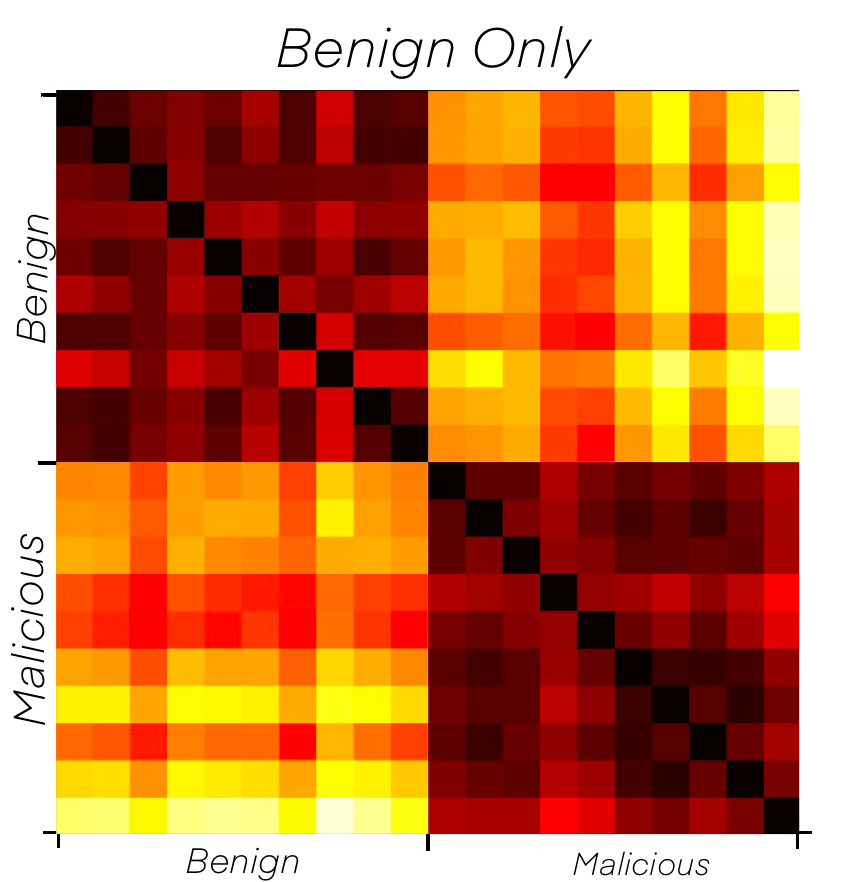
\includegraphics[width=0.2\textwidth]{jump_benign}\hspace{1em}%
    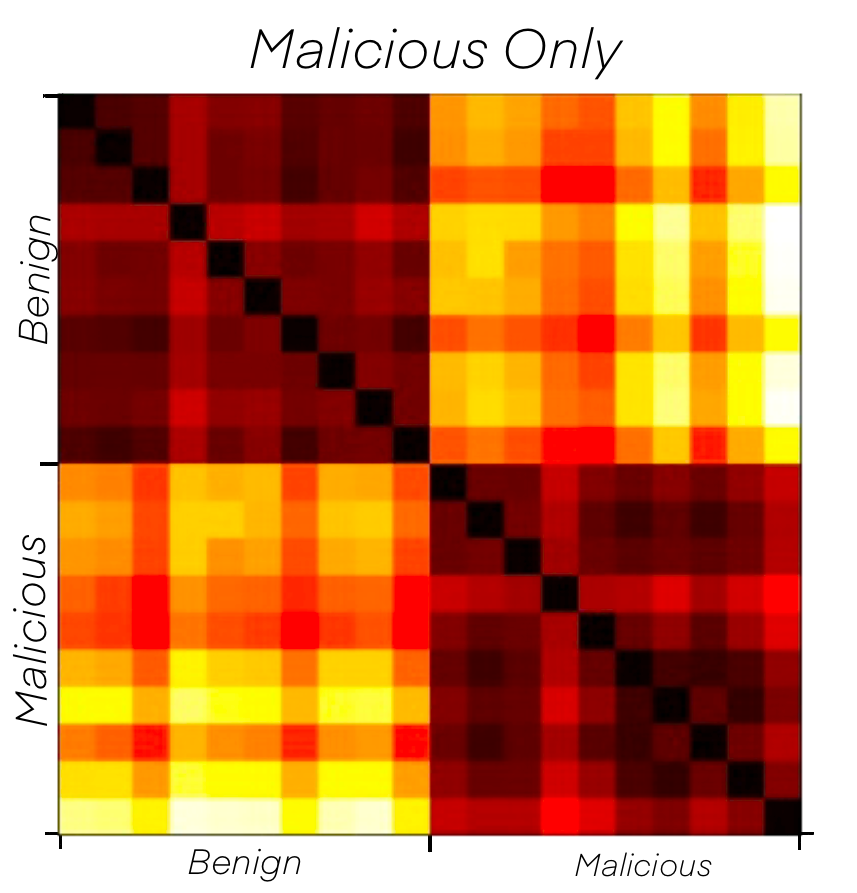
\includegraphics[width=0.2\textwidth]{jump_malicious}
    \centering
    \caption{
        Benign and Malicious Heatmaps
    }
%    \footnotesize{Heatmaps for 20 ground truth samples, 10 of each class. Cells of a darker color indicated lower
%        Kullback-Leibler Divergence values, while cells of a lighter color indicate higher KL Divergence values.}
    \label{fig:example_heatmaps}
\end{figure}


%    %! Author = jacobcarlson
%! Date = 4/26/23

\section{Model Selection}

Different models were tested, under the same input, to test the potential of using jump distributions to classify
malicious code samples. Multiple models were used throughout the testing off all opcode sets and KL divergence
method combinations. The python SciKit Learn framework was used to implement models, since it offers quick
implementation and reduces risk of manual error. The Linear SVM model was used as a ground truth due to simplicity.
Both Logistic Regression and the Multi-Layer Perception, MLP, Network were more accurate than the Linear SVM model.
When Logistic Regression and MLP Network were compared pairwise, under the same stipulations, the MLP network was more
accurate $(p=1.0)$.

\begin{table}[H]
    \begin{center}
        \begin{tabular}{l|S|S}
            \textbf{Model} & \textbf{Z} & \textbf{p}\\
            \hline
            Ridge Regression & -1.14 & 0.13\\
            Stochastic Gradient Descent & -46.13 & 0.00\\
            Logistic Regression & 13.34 & 1.00\\
            Multi-Layer Perceptron Network & 48.89 & 1.00\\
        \end{tabular}
        \label{tab:table1}
        \caption{Probability of Model being more accurate than Linear SVM}
        \footnotesize{Z scores and Probabilities of listed model being more accurate than a Scikit Learn’s Linear SVM
        when tested with a Wilcoxon Signed Rank test, using the differences between the accuracies of samples tested on
        the same data under the same conditions.}

    \end{center}
\end{table}

Scaling the data before inputting it into the model proved to result in a more accurate model, when each model was
compared its unscaled results. The scaled MLP network was also compared to all other scaled models, and no model was
determined to be more accurate.

\begin{table}[H]
    \begin{center}
        \begin{tabular}{l|S|S}
            \textbf{Model} & \textbf{Z} & \textbf{p}\\
            \hline
            Linear SVM & 11.73 & 1.00\\
            Ridge Regression & 23.36 & 1.00\\
            Logistic Regression & 8.22 & 1.00\\
            Multi-Layer Perceptron Network & 9.44 & 1.00\\
        \end{tabular}
        \label{tab:table2}
        \caption{Probability of Scaled Models being more accurate than non-Scaled Models}
        \footnotesize{Z scores and Probabilities of model being more accurate when data is scaled using SciKit Learns
        Standard Scaler than when data is not scaled, tested with a Wilcoxon Signed Rank test using the differences
        between the accuracies of samples tested on the same data under the same conditions.}

    \end{center}
\end{table}

\begin{table}[H]
    \begin{center}
        \begin{tabular}{l|S|S}
            \textbf{Model} & \textbf{Z} & \textbf{p}\\
            \hline
            Linear SVM & -50.76 & 0.00\\
            Logistic Regression & -51.59 & 0.00\\
            Stochastic Gradient Descent & -55.51 & 0.00\\
            Logistic Regression & -49.21 & 0.00\\
        \end{tabular}
        \centering
        \label{tab:table3}
        \caption{Probability of Scaled Models being more accurate than Scaled Multi-Layer Perceptron Network}
        \footnotesize{Z scores and Probabilities of model being more accurate than a scaled Multi-Layer Perceptron
        Network with a Wilcoxon Signed Rank test, using the differences between the accuracies of samples tested on the
        same data under the same conditions.}

    \end{center}
\end{table}

The Scaled Multi-Layer Perceptron Network was the most accurate under all parameter sets. This is not a novel finding,
as it had a much higher level of learnable parameters than the model it was compared against. The MLP Network had three
hidden layers ($[100, 200, 50]$) and ran for 300 iterations, the rest of the parameters were unchanged from SciKit Learn’s
default parameters. These parameter changes were decided purely because they were round numbers and larger than the
original input. These attributes are most likely not optimal, and the model could be refined to increase the overall
accuracy of the process, but similar to testing the granularity of the distribution, refining accuracy through standard
means is not the intention of this work.
    %! Author = jacobcarlson
%! Date = 4/26/23

\section{Opcode Set Collection}

The executables in the training set are all from machines running the Windows operating system,
primarily Windows 7\cite{lester}, but their opcode sets vary and a total of 1,457 different opcodes
were found in the training set.
Only $1.9\%$ of those opcodes occur in more than $25\%$ of the training samples, this means that most of the opcodes
will not make a difference when being used to make comparisons between files.
When an opcode does not occur, the distribution would just be uniform since there were no occurrences to
derive jumps from.
Comparing uniform distributions to ground truth distributions will not provide any meaningful information, so an effort
was made to find an optimal and commonly occurring set of opcodes.

\subsection{Benign, Malicious}

Simple opcode sets were derived by taking the $50$ most occurring opcodes from different sample sets of benign and
malicious files only.
This ensured that when creating distributions for individual executables, there was a good chance that most
of the opcodes had enough occurrences to yield a meaningful distribution.
$86\%$ of the opcodes overlapped between the two sets, so the distribution sets share most of the same data.
This reduces the chances of an opcode from one set being infrequent when compared against either opcode set.
The heatmaps in Figure \ref{fig:example_heatmaps}, display a consistent pattern of similarity between
ground truth samples of the same class over both classes in each opcode set heatmap.
The heatmaps look similar due to the number of overlapping opcodes in each set.

Table \ref{tab:benignMalicious} shows the average accuracies and standard deviations of the benign and malicious opcode
set when tested over 40 different combinations of ground truth and training samples.

\begin{table}[H]
    \begin{center}
        \captionsetup{justification=centering}
        \caption{Average Accuracy of Benign and Malicious Opcode Sets}
%        \footnotesize{Average test accuracies and standard deviations are obtained using ten different sample ground
%        truth sample pairs, tested 4 times each using a different random seed each time to differ the data. Resulting
%        in 40 different test cases.}
%        \footnotesize{$Bins: 100,\; KL\; Divergence\; Method: KL(X||dist),\; Model: MLP Scaled$\\}
        \begin{tabular}{c|c}
            \textbf{Benign} & \textbf{Malicious}\\
            \hline
            $88.1\% \pm 1.1\%$ & $88.7\% \pm 1.7\%$ \\
        \end{tabular}
        \label{tab:benignMalicious}
    \end{center}
\end{table}

The accuracies of each opcode set are not significantly different in terms of their average and standard deviations
(Figure \ref{tab:benignMalicious}); however, the malicious set was shown to be the more accurate set
$(Z=3.34, p=1.00)$, using a Wilcoxon Signed Rank test  where the input data is the difference between the
accuracies under the same conditions - $(KL\; Divergence\; Method:\; KL(X||dist))$,



\subsection{Union, Intersction, Disjoint}
Without using more in-depth approaches, the union, intersection, and disjoint of the benign and malicious opcode sets
were tested as opcode sets.
The union and intersection of the benign and malicious opcode sets only differ slightly from the original
sets, since those sets were so similar.
The benign and malicious sets each have seven opcodes that do not belong to the other set, so the benign and
malicious union set has $57$ opcodes while the intersection set has $43$ opcodes.
These sets both provide a valuable insight since the union set has more opcodes, which are frequent to at least one set,
while the intersection set has fewer opcodes, but they are all frequent to both opcode sets.

\begin{center}
    Benign - Intersection:\\
    $[abcb,\; cmpw,\; jns,\; lock,\; movzwl,\; sbbb,\; sete]$\\
    Malicious - Intersection:\\
    $[call,\; jmpl,\; leave,\; popl,\; retl,\; sarl,\; shll]$
\end{center}

When using the previously constructed sets the goal was to find opcodes that occurred frequently enough to create
a strong distribution, but the idea behind the disjoint set was to potentially use the lack of distribution to
illustrate difference, as was found in Bilar\cite{bilar}.
Opcodes that are common to malicious files but not benign files, and vice versa, were combined in the disjoint set.
Figure \ref{fig:unionIntersectionDisjoint}, introduces the heatmaps that show the summed KL Divergence values over all
opcodes in the union, intersection, and disjoint opcode sets.

\begin{figure}[H]
    \centering
    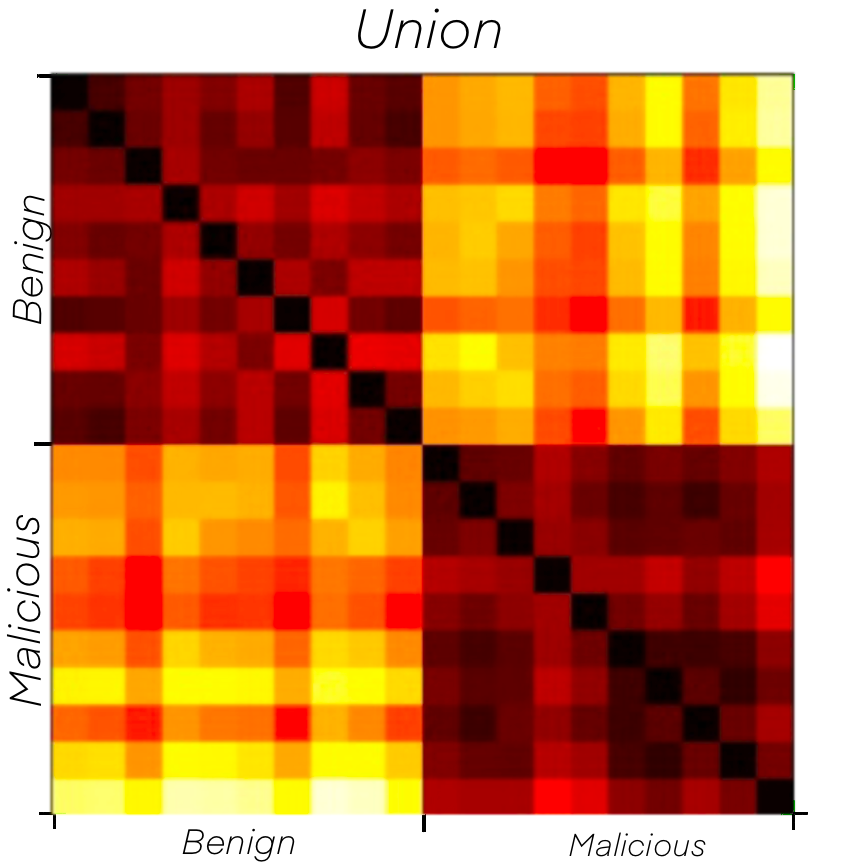
\includegraphics[width=0.2\textwidth]{jump_union}\hspace{1em}%
    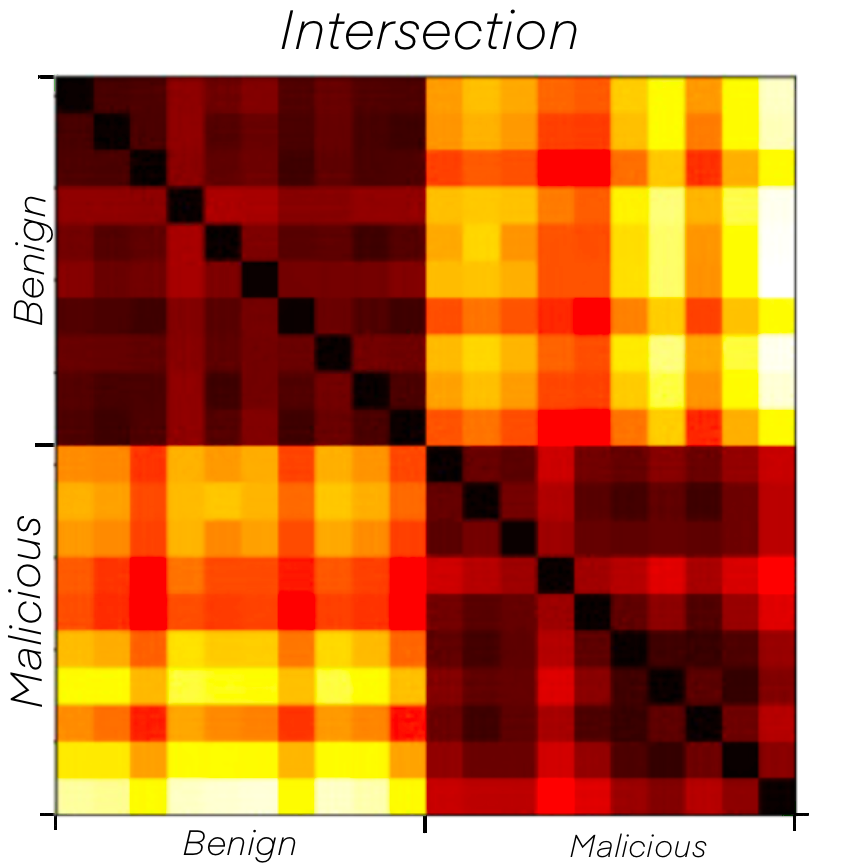
\includegraphics[width=0.2\textwidth]{jump_intersection}
    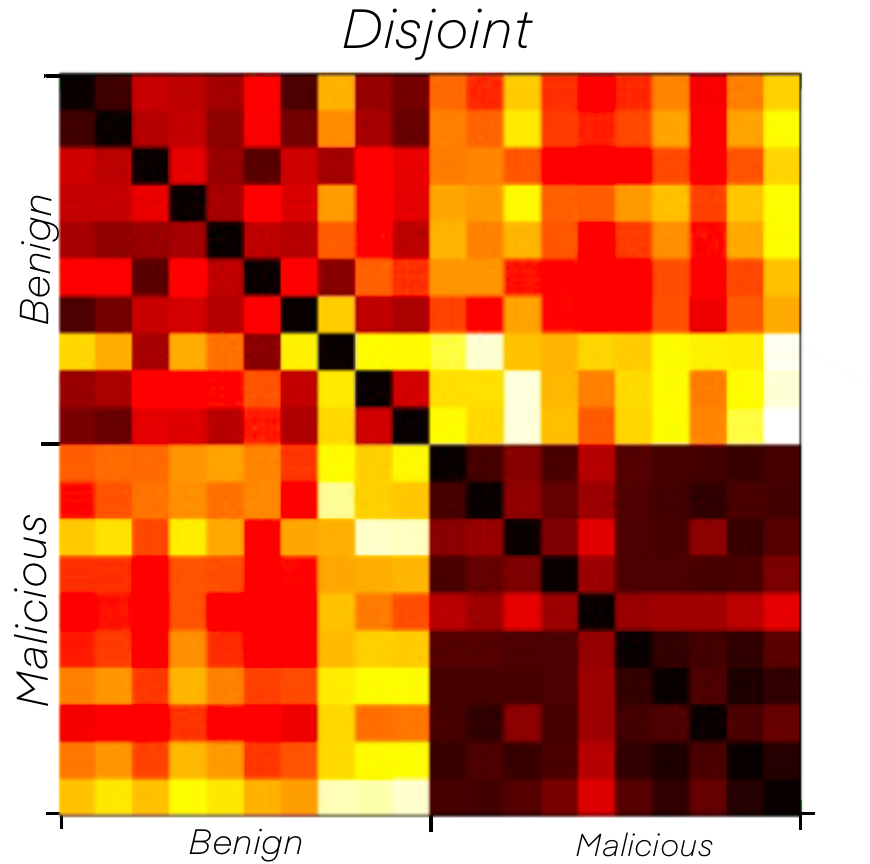
\includegraphics[width=0.2\textwidth]{jump_disjoint}
    \centering
    \caption{
        Union, Intersection, Disjoint Heatmaps
    }
%    \footnotesize{Heatmaps for 20 ground truth samples, 10 of each class. Cells of a darker color indicated lower
%    Kullback-Leibler Divergence values, while cells of a lighter color indicate higher KL Divergence values.}
    \label{fig:unionIntersectionDisjoint}
\end{figure}

The union and intersection opcode set heatmaps (Figure \ref{fig:unionIntersectionDisjoint}) each show a strong
degree of class similarity and intra-class dissimilarity.
This makes sense since both the malicious and benign classes heavily overlapped and also showed the same
characteristics.
This potential for increasingly different KL Divergence values when using infrequent opcodes is illustrated in
the disjoint heatmap (Figure \ref{fig:unionIntersectionDisjoint}), which does not follow as clear of a pattern
as the previous sets heatmaps.
There is a lower more consistent summed KL divergence between the malicious ground truth samples, while the Benign
samples seems to be much more erratic.

Table \ref{tab:unionInterectionDisjoint} shows the accuracies and standard deviations of the union, intersection,
and disjoint opcode sets when tested over 40 different combinations of ground truth and training samples.
Table \ref{tab:uidvsMalicious} compares the union, intersection, and disjoint opcode sets to malicious opcode set
under the same conditions, displaying the probability of the given opcode set being more accurate than the malicious
opcode set tested using the Wilcoxon Signed Rank Test.

%No opcode set was consistently more accurate than the malicious opcode set.

\begin{table}[H]
    \begin{center}
        \captionsetup{justification=centering}
        \caption{Average Accuracy of Union, Intersection, Disjoint Opcode Sets}
%        \footnotesize{Average test accuracies and standard deviations are obtained using ten different sample ground
%        truth sample pairs, tested 4 times each using a different random seed each time to differ the data. Resulting
%        in 40 different test cases.}
        \begin{tabular}{c|c|c}
            \textbf{Union} & \textbf{Intersection} & \textbf{Disjoint}\\
            \hline
            $88.6\% \pm 1.6\%$ & $88.0\% \pm 1.3\%$ & $84.9\% \pm 1.6\%$ \\
        \end{tabular}
        \label{tab:unionInterectionDisjoint}
%        \footnotesize{\\$KL\; Divergence\; Method: KL(X||dist)$}

    \end{center}
\end{table}

\begin{table}[H]
    \begin{center}
        \captionsetup{justification=centering}
        \caption{Probability of Opcode set yielding higher accuracy than Malicious Opcode Set}
%        \footnotesize{Z scores and Probabilities of opcode sets being more accurate than the malicious opcode set when
%        tested with a Wilcoxon Signed Rank test, using the differences between the accuracies of samples tested on the
%        same data under the same conditions.}
%        \footnotesize{\\$KL\; Divergence\; Method: KL(X||dist)$}
        \begin{tabular}{l|S|S}
            \textbf{Opcode Set} & \textbf{Z} & \textbf{p}\\
            \hline
            Union & -0.35 & 0.366\\
            Intersection & -3.28 & 0.000\\
            Disjoint & -5.28 & 0.000\\
        \end{tabular}
        \label{tab:uidvsMalicious}
    \end{center}
\end{table}

Out of the newly tested opcode sets, the union of the benign and malicious opcodes was the most accurate, but it still
failed to achieve a higher accuracy than the malicious opcode set.
The malicious opcode set is a subset of the union opcode set, meaning that the seven opcodes that are a part of
the benign set and not the malicious set do not provide any meaningful information and even decrease the accuracy when
compared to the malicious only opcode set.

While the intersection opcode set does not have the benign opcodes that seemingly decreased the accuracy of the
union set, it has a lower accuracy than both the malicious and union opcode sets.
Even though the differences in accuracy are minimal, the opcodes that belong to the malicious opcode
set seem to provide enough meaningful information to significantly boost accuracy.

The disjoint opcode set is much smaller than any of the other opcode sets that have been tested.
Disjoint had an interesting heatmap, showing strong similarity in the malicious opcode set, but had the lowest
accuracy by far.

The malicious opcode set group is the most accurate of the opcode set groups tested.
The malicious set being more accurate than the union opcode set, deters any further tests into opcode set size since
increasing the set size by $14\%$ failed to increase accuracy and any further size increases
will come with increased chance of infrequent opcodes.
The significantly worse accuracy, under $a=0.05$, of the intersection and disjoint sets also leads to the conclusion that
no further steps need to be taken to investigate opcodes that occur frequently in both sets (intersection) or
opcodes that only occur strongly in one set (disjoint).


    %! Author = jacobcarlson
%! Date = 4/27/23

\section{Kullback-Leibler Divergence Method Selection}

The Kullback-Leibler Divergence, $D_{KL} (p||q)$, measures the difference of distribution $p$ against distribution $q$
and will be used as the basis of comparison between distributions in this paper.
In the context of differentiating a set of distributions against a base standard, it made sense to consider the
distribution, or set of distributions, from the given file that we want to classify as $p$ and the ground truth
distribution sets as $q$.
This was how all previous accuracies were determined.

\subsection{Symmetric KL Divergence | Exploring Flipped Divergence}
$D_{KL}$ is asymmetric, and flipped $D_{KL}$  can be used to provide different insights than the standard method.
Flipping the KL Divergence, $D_{KL}(q||p)$, as well as taking the average of both options,
$(D_{KL}(p||q)+D_{KL}(q||p)) / 2$, provides alternative values that could provide different
and possible valuable information.
Table \ref{tab:kl1} shows the probability of the new KL Divergence methods being more accurate than $D_{KL}(q||p)$,
tested using the Wilcoxon Signed Rank test.
Both options have a high probability of being more accurate than $D_{KL}(x||dist)$, but neither are conclusively
better since they don’t meet the level of significance laid out in this test $(a=0.05)$.

\begin{table}[H]
    \begin{center}
        \captionsetup{justification=centering}
        \caption{Probability of KL Divergence method yielding higher accuracy than $D_{KL}(x||dist)$}
%        \footnotesize{Z scores and Probabilities of a more accurate model when using a different KL Divergence
%        method compared to $D_{KL}(x||dist)$, using the differences between the accuracies of samples tested on the
%        same data under the same conditions.}
%        \footnotesize{\\$Opcode Set: Malicious Only,$}
        \begin{tabular}{l|S|S}
            \textbf{KL Method} & \textbf{Z} & \textbf{p}\\
            \hline
            $D_{KL}(dist||x)$ & 0.98 & 0.837\\
            Symmetric & 1.06 & 0.856\\
        \end{tabular}
        \label{tab:kl1}
    \end{center}
\end{table}

\subsection{Logarithm Mapping KL Divergence Values}
KL Divergence values range from zero, when two distributions are exactly alike, to infinity, when distributions
share no similarity.
While the KL divergence values derived from these distributions fall in a much smaller range with an upper bound
near $~10$.
Machine learning algorithms typically perform better when input data is normalized to a standard range\cite{singh}.
To normalize and more evenly distribute the data, the KL Divergence value was mapped using $log_{10}$ to put almost
all the data in between $-1$ and $+1$.

On the lower bound, no samples were similar enough to a ground truth distribution to result in a KL Divergence
of less than $.1$, so no samples passed the lower bound of $-1$.
Any KL Divergence value that was greater than $10$ will pass the soft boundary of $+1$ after mapped.
The number of upper bound outliers is minimal and these values do not range very far above $10$.
Any outliers will be very close to $+1$ so none of these outliers are significant.
Most data ends up within a range of $-1$ and $+1$ so outliers were not a very large concern.

Table \ref{tab:mapComparisons} shows the probability of the accuracy being higher using the transformation $log_{10}$ on
KL Divergence against the lack of a transformation.

\begin{table}[H]
    \begin{center}
        \captionsetup{justification=centering}
        \caption{Probability that taking the $log_{10}$ of the KL Divergence result in higher Accuracy}
%        \footnotesize{Z scores and Probabilities of a higher accuracy when taking the $log_{10}$ of the KL Divergence
%            before being used as input for the model, using the differences between the accuracies of samples tested
%        on the same data under the same conditions.}
%        \footnotesize{\\$Opcode\; Set: Malicious\; Only$}
        \begin{tabular}{l|S|S}
            \textbf{KL Method} & \textbf{Z} & \textbf{p}\\
            \hline
            $D_{KL}(x||dist)$ & -0.75 & 0.226\\
            $D_{KL}(dist||x)$ & 0.79 & 0.786\\
            Symmetric & 0.61 & 0.730\\
        \end{tabular}
        \label{tab:mapComparisons}

    \end{center}
\end{table}

Taking the $log_{10}$ of KL Divergence values did not provide a significant enough increase in accuracy when
compared to the same KL Divergence with no transformation.

The flipped and symmetric accuracies had above a $84\%$ probability of being more accurate than $D_{KL}(x||dist)$
and both methods had above a $73\%$ probability of being more accurate when used with a transformation.
While neither parameter was significantly more accurate on its own, they were combined and tested against
$D_{KL}(x||dist)$ in Table \ref{tab:xdistComparison}

\begin{table}[H]
    \begin{center}
        \captionsetup{justification=centering}
        \caption{Probability of KL transformations \\against $D_{KL}(x||dist)$}
%        \footnotesize{Z scores and Probabilities of different KL divergence methods being more accurate than
%            $D_{KL}(x||dist)$, using the differences between the accuracies of samples tested on the same data
%            under the same conditions.}
%        \footnotesize{\\$Opcode\; Set: Malicious\; Only$}
        \begin{tabular}{l|S|S}
            \textbf{KL Method} & \textbf{Z} & \textbf{p}\\
            \hline
            $log_{10}(D_{KL}(dist||x))$ & 2.18 & 0.985\\
            $log_{10}(Symmetric)$ & 0.78 & 0.784\\
        \end{tabular}
        \label{tab:xdistComparison}
    \end{center}
\end{table}

$log_{10}(D_{KL}(dist||x))$ proved to be more accurate than $D_{KL}(x||dist)$ with a high level of significance
when compared with the Wilcoxon signed rank test in Table \ref{tab:xdistComparison}.
$log_{10}(D_{KL}(dist||x))$ will now be the primary KL Divergence method.

This did not change any findings made in the previous sections.
While the accuracies of the opcode tests increased they did so consistently across all opcodes sets
and did not change how they compare.




    %! Author = jacobcarlson
%! Date = 4/27/23

\section{Test Results and Conclusion}

The final model was tested against multiple datasets which were not used to train or verify any models.
A set of benign files was obtained from analyzing all files with a $.exe$ extension on a clean install of a Windows 10
virtual machine.

Three malicious file sets were downloaded from VirusShare\cite{virusShare1,virusShare5,virusShare451}, an online malware repository for security researchers.
Each file set had over $130,000$  malware samples, but only $15,000$ executables were used from each set due to
processing time constraints.
The first two datasets from VirusShare ($VirusShare\_00000$ and $VirusShare\_00005$) were written in 2012,
while $VirusShare\_00451$ was written more recently.
These malicious files are curated from user submissions, so there is reason to believe that most of the files in
$VirusShare\_00451$ are from current systems.

A final benign set was obtained from a macbook running macOS Big Sur, by analyzing all executable files
that had $.bundle$, $.dylib$, or $.so$ extensions.
Table \ref{tab:testTable} shows the average accuracy of each test set, which is tested on $40$ models each trained
against different combinations of ground truth and training samples with $250$ random selected samples from each test
used to determine the accuracy.



\begin{center}
    \underline{Final Model Parameters}\\
    Opcode Set - Malicious Only\\
    KL Divergence - $log_{10}(D_{KL}(dist||x))$\\
    Bins - 100\\
    Model - Multi-Layer Perceptron, \\
    \footnotesize{Scaled Input}
    \footnotesize{hidden layers - [100, 200, 50]}
\end{center}


\begin{table}[H]
    \begin{center}
        \captionsetup{justification=centering}
        \caption{Average Accuracy of models on purely Test Datasets}
%        \footnotesize{Test accuracies and standard deviations are obtained using ten different samples ground truth
%        sample pairs, tested 4 times each using a different random seed each time to differ the data.
%        Resulting in 40 different test cases.}
%        \footnotesize{\\$Opcode\; Set: Malicious Only$\\$KL\; Divergence\; Method: log_{10}(D_{KL}(dist||x))$}
        \begin{tabular}{l|l|r}
            \textbf{Sample Set} & \textbf{Class} & \textbf{Accuracy}\\
            \hline
            Windows10 Virtual & Benign & $79.3\% \pm 5.8\%$\\
            VirusShare\_00000 & Malicious & $98.4\% \pm 0.9\%$\\
            VirusShare\_00005 & Malicious & $97.5\% \pm 1.3\%$\\
            VirusShare\_00451 & Malicious & $94.7\% \pm 3.5\%$\\
            MacOS Big Sur & Benign & $35.8\% \pm 4.4\%$\\
        \end{tabular}
        \label{tab:testTable}
    \end{center}
\end{table}

The malicious data sets were more accurate than the accuracies from validation sets during training,
while the benign samples faltered below that accuracy.
The weighted average of the accuracies is almost identical to that of the tests conducted on these models during training
when ignoring the MacOS files.
There was no reason to believe that the MacOS files would be accurately classified when using a model trained on
executable obtained from a Window’s 7 operating system\cite{lester}, but the fact that it had an accuracy
less than a random decision maker would suggest that there is data to be learned from the MacOS
samples, it just does not correlate with the windows data.

The increase in accuracy over the Malicious data sets could be due to the difference in samples under the
training set and test sets.
The training set classifies malicious files based of whether multiple antivirus software identifies it as
malicious\cite{lester}, while VirusShare is cultivated by a digital forensics team\cite{virusShare1,virusShare5,virusShare451}.
This more hands on approach could mean that the malicious samples in the test set are more malicious and differ more
from benign files than the malicious samples in training did.

The more recent VirusShare sample was less accurate than the older VirusShare samples.
The models were trained on Windows 7 files\cite{lester}, which was the most popular windows operating system at the
time the older VirusShare sets were curated\cite{statcounter}.
The models most likely performed very strongly on malicious code from Windows 7 Operating Systems since that what
it was trained on, it is even possible that there is overlap between samples but there is no way to verify that.
Similar logic could be used to attribute the low accuracy of the Windows 10 samples.


    \appendix
%    \bibliographystyle{plain}
    \printbibliography
\end{document}